\documentclass{article}
\usepackage[utf8]{inputenc}
\title{Machine Learning:  Assignment 2}
\author{Karsten Standnes - STNKAR012}
\date{October 2017}

\usepackage{natbib}
\usepackage{graphicx}
\usepackage{enumitem}
\usepackage{multirow}
\usepackage{float}
\usepackage[a4paper, total={6in, 9in}]{geometry}
\usepackage{attachfile}
\usepackage{hyperref}
\usepackage{color}
\usepackage{mathtools}
\usepackage{hyperref}
\usepackage{amsmath}
\usepackage{amssymb}
\usepackage{amsfonts}
\usepackage{listings}
\usepackage{tikz}
\usepackage{svg}
\tikzset{fontscale/.style = {font=\relsize{#1}}
    }

\lstset{language=R,
    basicstyle=\small\ttfamily,
    stringstyle=\color{DarkGreen},
    otherkeywords={0,1,2,3,4,5,6,7,8,9},
    morekeywords={TRUE,FALSE},
    deletekeywords={data,frame,length,as,character},
    keywordstyle=\color{blue},
    commentstyle=\color{DarkGreen},
    breaklines = true,
    language=R,
    numbers=left,
    numberstyle=\ttfamily\color{gray}\footnotesize,
    stepnumber=1,
    numbersep=5pt,
    backgroundcolor=\color{white},
    showspaces=false,
    showstringspaces=false,
    showtabs=false,
    frame=leftline,
    tabsize=4,
    captionpos=b,
    breakatwhitespace=false,
    title=\lstname,
    escapeinside={},
    keywordstyle={},
    morekeywords={}
}

\begin{document}

\maketitle
\setlength\parindent{0pt}

\section{Introduction}

In the world today there are many methods that fall under the category of "Machine
Learning", some being very simular and some very different. All of them share in common
that they use data to produce a model that can be used on unseen data. When sucessful this
is very appeling in todays society when we got lots of data on situations where there is likely
to be a underlying pattern, another requirement for learning. There is broad agreement
that machine learning is a good way to make prediction and classification models, and often
the only computational feasible way. This makes it a task to decide which method in
machine learning to chose for a given problem. The answer is not always the same and
several methods can be good, but for different reasons. In this task I will show several
different machine learning algortihms and how they perform on classifying pictures
of handwritten numbers.

\section{Methods}

\subsection{Tree based methods}



\subsection{Neural Networks}
For Neural Networks I have decided to use a convulutional neural network because of
it great performance in problems that can be represented as an "image". This because it
convolutional neural networks(CNN's) works by recognizing paterns in images or represented as
a matrix or tensor(multidimension matrix) in the computer. It does so by using convolutional,
pooling and voting layers. Multiple of these can be stacked to create a very a precise recongising
images.

\begin{figure}[H]
    \centering
        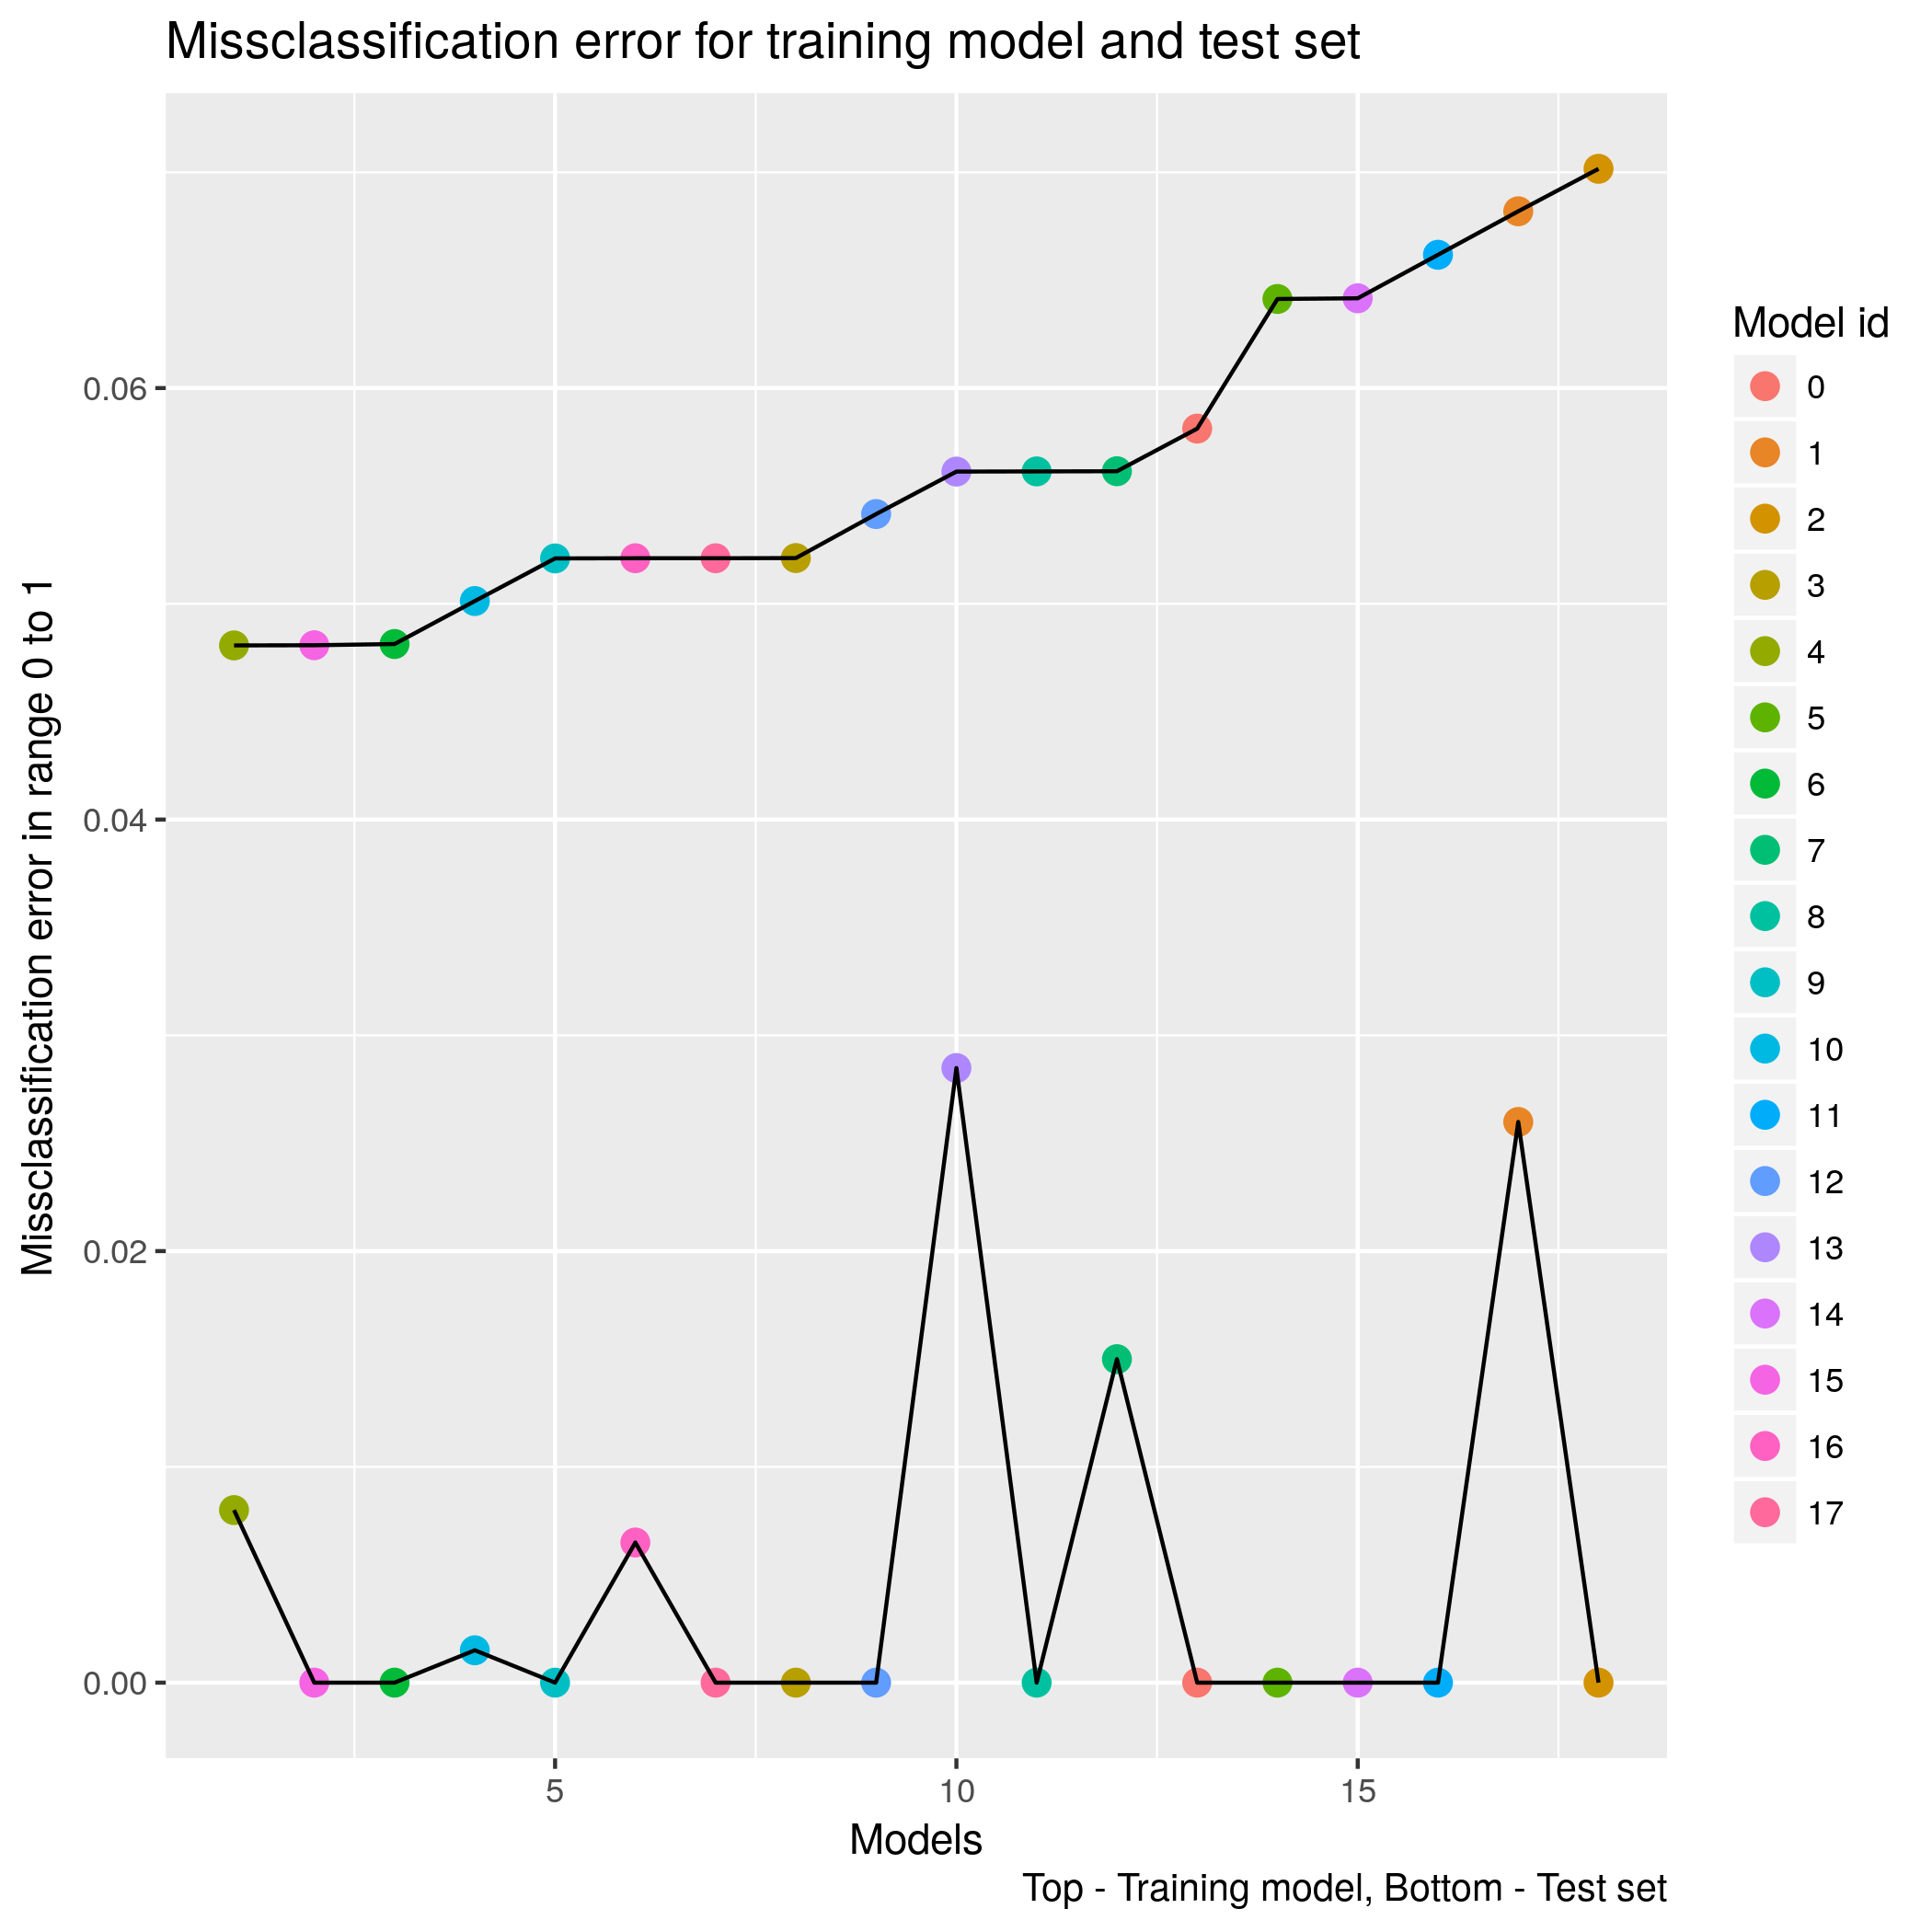
\includegraphics[width =.9\linewidth]{../R_scripts/Neural_Networks/results_NN/per_class_error.png}
    \caption{Error measures $E_{out}$ and $E_{val}$ are plotted for different sizes of training and validation sets.}
  \label{plot:1ii}
\end{figure}


\subsection{Support vector machines}

\section{Results}

\section{Discussion}

\section{Acknowledgments}

\section{Appendices}

\end{document}
